% ChatGPT Directions 0 :
% This is a Tbox Problem set for the following standards: 7.RP.A.2a, 7.RP.A.2b 
%--------------------------------------------------
\documentclass[10pt]{article}
\usepackage[a4paper, top=0.8in, bottom=0.7in, left=0.8in, right=0.8in]{geometry}
\usepackage{amsmath}
\usepackage{amsfonts}
\usepackage{latexsym}
\usepackage{graphicx}
\usepackage{fancyhdr}
\usepackage{tcolorbox}
\usepackage{enumitem}
\usepackage{setspace}
\usepackage{pgfplots}
\usepackage{tikz}
\usepackage[defaultfam,tabular,lining]{montserrat} % Font settings for Montserrat

% General Comment: Template for creating problem sets in a structured format with headers, titles, and sections.
% This document uses Montserrat font and consistent styles for exercises, problems, and performance tasks.

% -------------------------------------------------------------------
\setlength{\parindent}{0pt}
\pagestyle{fancy}

\setlength{\headheight}{27.11148pt}
\addtolength{\topmargin}{-15.11148pt}

\fancyhf{}
%\fancyhead[L]{\textbf{7.RP.A.2a, 7.RP.A.2b: Understanding Proportional Relationships - Answer Key}}
\fancyhead[R]{
\includegraphics[width=0.8cm]{Round Logo.png}} % Placeholder for logo
\fancyfoot[C]{\footnotesize © Study Smart Tutors}

\sloppy

\newcommand{\dsfrac}[2]{\dfrac{#1}{#2}} % New command for display style fractions
\pgfplotsset{compat=1.18} 

\begin{document}

\subsection*{Problem Set: Understanding Proportional Relationships - Answer Key}
\onehalfspacing

% Learning Objective Box
\begin{tcolorbox}[colframe=black!40, colback=gray!5, 
coltitle=black, colbacktitle=black!20, fonttitle=\bfseries\Large, 
title=Learning Objective, halign title=center, left=5pt, right=5pt, top=5pt, bottom=15pt]
\textbf{Objective:} Solve problems involving proportional relationships and represent these relationships using equations with variables.
\end{tcolorbox}

% Exercises Box
\begin{tcolorbox}[colframe=black!60, colback=white, 
coltitle=black, colbacktitle=black!15, fonttitle=\bfseries\Large, 
title=Exercises, halign title=center, left=10pt, right=10pt, top=10pt, bottom=35pt]
\begin{enumerate}[itemsep=2em]
    \item Find the unit rate: \( \dsfrac{84}{7} \).\\
    \textcolor{red}{\textbf{Solution:} \( 84 \div 7 = 12 \). The unit rate is \( 12 \).}

    \item Write an equation for the relationship: "If 3 apples cost \$6, how much will \(x\) apples cost?"\\
    \textcolor{red}{\textbf{Solution:} \( C = 2x \), where \(C\) is the cost, and \(x\) is the number of apples.}

    \item Solve: \(4x = 48\).\\
    \textcolor{red}{\textbf{Solution:} Divide both sides by 4: \(x = 48 \div 4 = 12\). Final answer: \(x = 12\).}

    \item Complete the table for the proportional relationship:
    \newline 
    \begin{tabular}{|c|c|}
        \hline
        Number of Items & Cost (in \$) \\ \hline
        2 & 10 \\ \hline
        5 & \textcolor{red}{25} \\ \hline
        8 & \textcolor{red}{40} \\ \hline
    \end{tabular}\\
    \textcolor{red}{\textbf{Solution:} The cost per item is \(10 \div 2 = 5\). Multiply the number of items by 5 to complete the table.}

    \item A machine produces 120 widgets in 4 hours. Find the rate of production (widgets per hour).\\
    \textcolor{red}{\textbf{Solution:} \(120 \div 4 = 30\). The rate of production is \(30 \, \text{widgets per hour}\).}

    \item Determine if the following table represents a proportional relationship. If yes, write the equation. If not, explain why not. \\
    \newline
    \begin{tabular}{|c|c|}
        \hline
        \(x\) & \(y\) \\ \hline
        1 & 3 \\ \hline
        2 & 6 \\ \hline
        3 & 9 \\ \hline
        4 & 11 \\ \hline
    \end{tabular}\\
    \textcolor{red}{\textbf{Solution:} The relationship is not proportional because the ratio \( \frac{y}{x} \) is not constant. For example, \( \frac{9}{3} = 3 \), but \( \frac{11}{4} \neq 3 \).}

    \item If \(y\) is proportional to \(x\), and \(y = 24\) when \(x = 6\), find the constant of proportionality \(k\). Write the equation.\\
    \textcolor{red}{\textbf{Solution:} \(k = \frac{y}{x} = \frac{24}{6} = 4\). The equation is \(y = 4x\).}
\end{enumerate}
\end{tcolorbox}

\vspace{1em}

% Problems Box
\begin{tcolorbox}[colframe=black!60, colback=white, 
coltitle=black, colbacktitle=black!15, fonttitle=\bfseries\Large, 
title=Problems, halign title=center, left=10pt, right=10pt, top=10pt, bottom=30pt]
\begin{enumerate}[start=9, itemsep=3em]
    \item A car travels 180 miles in 3 hours. 
    \begin{enumerate}[label=(\alph*)]
        \item Find the speed of the car (miles per hour).\\
        \textcolor{red}{\textbf{Solution:} \(180 \div 3 = 60 \, \text{miles per hour}\).}

        \item Write an equation for the total distance \(d\) as a function of time \(t\).\\
        \textcolor{red}{\textbf{Solution:} \(d = 60t\).}
    \end{enumerate}

    \item A store sells 4 bags of rice for \$20.  
    \begin{enumerate}[label=(\alph*)]
        \item Write an equation for the total cost \(C\) as a function of the number of bags \(x\).\\
        \textcolor{red}{\textbf{Solution:} \(C = 5x\), where \(x\) is the number of bags.}

        \item Determine the cost for 7 bags of rice.\\
        \textcolor{red}{\textbf{Solution:} \(C = 5 \times 7 = 35\). The cost is \$35.}
    \end{enumerate}

    \item A recipe uses 3 cups of flour to make 6 servings.  
    \begin{enumerate}[label=(\alph*)]
        \item Find the constant of proportionality.\\
        \textcolor{red}{\textbf{Solution:} \(k = \frac{3}{6} = 0.5\).}

        \item How many cups of flour are needed to make 12 servings?\\
        \textcolor{red}{\textbf{Solution:} \(Cups = 0.5 \times 12 = 6 \, \text{cups}\).}
    \end{enumerate}

    \item Graph the proportional relationship represented by the equation \(y = 3x\).\\
    \begin{center}
    \begin{tikzpicture}[scale=0.4]
        % Draw axes
        \draw[thick,->] (-0.5,0) -- (5.5,0) node[right]{\(x\)};
        \draw[thick,->] (0,-0.5) -- (0,13) node[above]{\(y\)};

        % Grid and ticks
        \draw[help lines, color=gray!30] (0,0) grid (5,12);
        \foreach \x in {0,1,2,3,4,5} \draw (\x,0) -- (\x,-0.2) node[below]{\x};
        \foreach \y in {0,3,6,9,12} \draw (0,\y) -- (-0.2,\y) node[left]{\y};

        % Plot the points
        \foreach \x in {1,2,3,4} {
            \fill[red] (\x,3*\x) circle (2.5pt);
        }

        % Draw the line
        \draw[thick,red] (0,0) -- (4,12);
    \end{tikzpicture}
\end{center}


\end{enumerate}
\end{tcolorbox}

% Performance Task Box
\vspace{1em}
\begin{tcolorbox}[colframe=black!60, colback=white, 
coltitle=black, colbacktitle=black!15, fonttitle=\bfseries\Large, 
title=Performance Task: Planning a Shopping Trip, halign title=center, left=10pt, right=10pt, top=10pt, bottom=80pt]
You are shopping for school supplies. Here’s what you know:
\begin{itemize}
    \item Notebooks cost \$3 each.
    \item Pencils are \$0.50 each.
    \item You have a budget of \$30.
\end{itemize}
\textbf{Task:}
\begin{enumerate}[itemsep=4em]
    \item Write an equation to represent the total cost of buying \(n\) notebooks and \(p\) pencils.\\
    \textcolor{red}{\textbf{Solution:} \(C = 3n + 0.5p\), where \(C\) is the total cost.}

    \item Determine how many notebooks and pencils you can buy if you spend exactly \$30.\\
    \textcolor{red}{\textbf{Solution:} Solve \(3n + 0.5p = 30\) for different values of \(n\) and \(p\) (e.g., \(n = 5, p = 10\)).}

    \item Design a plan to maximize the number of items purchased while staying within budget.\\
    \textcolor{red}{\textbf{Solution:} Maximize \(n + p\) under the constraint \(3n + 0.5p = 30\). For example, \(n = 5, p = 20\).}
\end{enumerate}
\end{tcolorbox}

% Reflection Box
\vspace{1em}
\begin{tcolorbox}[colframe=black!60, colback=white, 
coltitle=black, colbacktitle=black!15, fonttitle=\bfseries\Large, 
title=Reflection, halign title=center, left=10pt, right=10pt, top=10pt, bottom=110pt]
What strategies did you use to solve the performance task? How does identifying proportional relationships help in solving real-world problems? Share any patterns or observations.
\end{tcolorbox}

\end{document}
